\documentclass{ximera}

%\usepackage{todonotes}

\newcommand{\todo}{}

\usepackage{esint} % for \oiint
\graphicspath{
  {./}
  {ximeraTutorial/}
}

\newcommand{\mooculus}{\textsf{\textbf{MOOC}\textnormal{\textsf{ULUS}}}}

\usepackage{tkz-euclide}
\tikzset{>=stealth} %% cool arrow head
\tikzset{shorten <>/.style={ shorten >=#1, shorten <=#1 } } %% allows shorter vectors

\usetikzlibrary{backgrounds} %% for boxes around graphs
\usetikzlibrary{shapes,positioning}  %% Clouds and stars
\usetikzlibrary{matrix} %% for matrix
\usepgfplotslibrary{polar} %% for polar plots
\usetkzobj{all}
\usepackage[makeroom]{cancel} %% for strike outs
%\usepackage{mathtools} %% for pretty underbrace % Breaks Ximera
\usepackage{multicol}
\usepackage{pgffor} %% required for integral for loops


%% http://tex.stackexchange.com/questions/66490/drawing-a-tikz-arc-specifying-the-center
%% Draws beach ball 
\tikzset{pics/carc/.style args={#1:#2:#3}{code={\draw[pic actions] (#1:#3) arc(#1:#2:#3);}}}



\usepackage{array}
\setlength{\extrarowheight}{+.1cm}   
\newdimen\digitwidth
\settowidth\digitwidth{9}
\def\divrule#1#2{
\noalign{\moveright#1\digitwidth
\vbox{\hrule width#2\digitwidth}}}





\newcommand{\RR}{\mathbb R}
\newcommand{\R}{\mathbb R}
\newcommand{\N}{\mathbb N}
\newcommand{\Z}{\mathbb Z}

\newcommand{\sagemath}{\textsf{SageMath}}


%\renewcommand{\d}{\,d\!}
\renewcommand{\d}{\mathop{}\!d}
\newcommand{\dd}[2][]{\frac{\d #1}{\d #2}}
\newcommand{\pp}[2][]{\frac{\partial #1}{\partial #2}}
\renewcommand{\l}{\ell}
\newcommand{\ddx}{\frac{d}{\d x}}

\newcommand{\zeroOverZero}{\ensuremath{\boldsymbol{\tfrac{0}{0}}}}
\newcommand{\inftyOverInfty}{\ensuremath{\boldsymbol{\tfrac{\infty}{\infty}}}}
\newcommand{\zeroOverInfty}{\ensuremath{\boldsymbol{\tfrac{0}{\infty}}}}
\newcommand{\zeroTimesInfty}{\ensuremath{\small\boldsymbol{0\cdot \infty}}}
\newcommand{\inftyMinusInfty}{\ensuremath{\small\boldsymbol{\infty - \infty}}}
\newcommand{\oneToInfty}{\ensuremath{\boldsymbol{1^\infty}}}
\newcommand{\zeroToZero}{\ensuremath{\boldsymbol{0^0}}}
\newcommand{\inftyToZero}{\ensuremath{\boldsymbol{\infty^0}}}



\newcommand{\numOverZero}{\ensuremath{\boldsymbol{\tfrac{\#}{0}}}}
\newcommand{\dfn}{\textbf}
%\newcommand{\unit}{\,\mathrm}
\newcommand{\unit}{\mathop{}\!\mathrm}
\newcommand{\eval}[1]{\bigg[ #1 \bigg]}
\newcommand{\seq}[1]{\left( #1 \right)}
\renewcommand{\epsilon}{\varepsilon}
\renewcommand{\phi}{\varphi}


\renewcommand{\iff}{\Leftrightarrow}

\DeclareMathOperator{\arccot}{arccot}
\DeclareMathOperator{\arcsec}{arcsec}
\DeclareMathOperator{\arccsc}{arccsc}
\DeclareMathOperator{\si}{Si}
\DeclareMathOperator{\proj}{\vec{proj}}
\DeclareMathOperator{\scal}{scal}
\DeclareMathOperator{\sign}{sign}


%% \newcommand{\tightoverset}[2]{% for arrow vec
%%   \mathop{#2}\limits^{\vbox to -.5ex{\kern-0.75ex\hbox{$#1$}\vss}}}
\newcommand{\arrowvec}{\overrightarrow}
%\renewcommand{\vec}[1]{\arrowvec{\mathbf{#1}}}
\renewcommand{\vec}{\mathbf}
\newcommand{\veci}{{\boldsymbol{\hat{\imath}}}}
\newcommand{\vecj}{{\boldsymbol{\hat{\jmath}}}}
\newcommand{\veck}{{\boldsymbol{\hat{k}}}}
\newcommand{\vecl}{\boldsymbol{\l}}
\newcommand{\uvec}[1]{\mathbf{\hat{#1}}}
\newcommand{\utan}{\mathbf{\hat{t}}}
\newcommand{\unormal}{\mathbf{\hat{n}}}
\newcommand{\ubinormal}{\mathbf{\hat{b}}}

\newcommand{\dotp}{\bullet}
\newcommand{\cross}{\boldsymbol\times}
\newcommand{\grad}{\boldsymbol\nabla}
\newcommand{\divergence}{\grad\dotp}
\newcommand{\curl}{\grad\cross}
%\DeclareMathOperator{\divergence}{divergence}
%\DeclareMathOperator{\curl}[1]{\grad\cross #1}
\newcommand{\lto}{\mathop{\longrightarrow\,}\limits}

\renewcommand{\bar}{\overline}

\colorlet{textColor}{black} 
\colorlet{background}{white}
\colorlet{penColor}{blue!50!black} % Color of a curve in a plot
\colorlet{penColor2}{red!50!black}% Color of a curve in a plot
\colorlet{penColor3}{red!50!blue} % Color of a curve in a plot
\colorlet{penColor4}{green!50!black} % Color of a curve in a plot
\colorlet{penColor5}{orange!80!black} % Color of a curve in a plot
\colorlet{penColor6}{yellow!70!black} % Color of a curve in a plot
\colorlet{fill1}{penColor!20} % Color of fill in a plot
\colorlet{fill2}{penColor2!20} % Color of fill in a plot
\colorlet{fillp}{fill1} % Color of positive area
\colorlet{filln}{penColor2!20} % Color of negative area
\colorlet{fill3}{penColor3!20} % Fill
\colorlet{fill4}{penColor4!20} % Fill
\colorlet{fill5}{penColor5!20} % Fill
\colorlet{gridColor}{gray!50} % Color of grid in a plot

\newcommand{\surfaceColor}{violet}
\newcommand{\surfaceColorTwo}{redyellow}
\newcommand{\sliceColor}{greenyellow}




\pgfmathdeclarefunction{gauss}{2}{% gives gaussian
  \pgfmathparse{1/(#2*sqrt(2*pi))*exp(-((x-#1)^2)/(2*#2^2))}%
}


%%%%%%%%%%%%%
%% Vectors
%%%%%%%%%%%%%

%% Simple horiz vectors
\renewcommand{\vector}[1]{\left\langle #1\right\rangle}


%% %% Complex Horiz Vectors with angle brackets
%% \makeatletter
%% \renewcommand{\vector}[2][ , ]{\left\langle%
%%   \def\nextitem{\def\nextitem{#1}}%
%%   \@for \el:=#2\do{\nextitem\el}\right\rangle%
%% }
%% \makeatother

%% %% Vertical Vectors
%% \def\vector#1{\begin{bmatrix}\vecListA#1,,\end{bmatrix}}
%% \def\vecListA#1,{\if,#1,\else #1\cr \expandafter \vecListA \fi}

%%%%%%%%%%%%%
%% End of vectors
%%%%%%%%%%%%%

%\newcommand{\fullwidth}{}
%\newcommand{\normalwidth}{}



%% makes a snazzy t-chart for evaluating functions
%\newenvironment{tchart}{\rowcolors{2}{}{background!90!textColor}\array}{\endarray}

%%This is to help with formatting on future title pages.
\newenvironment{sectionOutcomes}{}{} 



%% Flowchart stuff
%\tikzstyle{startstop} = [rectangle, rounded corners, minimum width=3cm, minimum height=1cm,text centered, draw=black]
%\tikzstyle{question} = [rectangle, minimum width=3cm, minimum height=1cm, text centered, draw=black]
%\tikzstyle{decision} = [trapezium, trapezium left angle=70, trapezium right angle=110, minimum width=3cm, minimum height=1cm, text centered, draw=black]
%\tikzstyle{question} = [rectangle, rounded corners, minimum width=3cm, minimum height=1cm,text centered, draw=black]
%\tikzstyle{process} = [rectangle, minimum width=3cm, minimum height=1cm, text centered, draw=black]
%\tikzstyle{decision} = [trapezium, trapezium left angle=70, trapezium right angle=110, minimum width=3cm, minimum height=1cm, text centered, draw=black]


\title{Grocery Store Function}

\begin{document}

\begin{abstract}
%Stuff can go here later if we want!
\end{abstract}

\maketitle

\textbf{The Product-Price Relation}



\[
\begin{array}{|l|l|l|}
\hline
(102707849467, 1.24) & (151603090297, 1.28) & (147882057258, 1.33) \\\hline
(121219574901, 3.95) & (196997564303, 4.61) & (120984686834, 1.39) \\\hline
(192107524489, 3.06) & (116532522722, 5.46) & (190132246907, 1.24) \\\hline
(105853328761, 1.33) & (185066339518, 1.25) & (178355581117, 4.81) \\\hline 
(139647551818, 0.79) & (182604889507, 2.07) & (163639788196, 0.95) \\\hline 
(151593345667, 2.07) & (173630558604, 1.24) & (141821520319, 1.25) \\\hline 
(142144767669, 3.38) & (187266863018, 2.63) & (146494777598, 1.33) \\\hline 
(155152532584, 3.06) & (159664504967, 0.79) & (137707844901, 3.67) \\\hline 
(116506724164, 2.17) & (139411323037, 1.71) & (127419334209, 1.90) \\\hline 
(120957405055, 4.66) & (133860480889, 1.39) & (145242561846, 0.79) \\\hline 
(105756538007, 0.95) & (162440197320, 1.46) & (198053092474, 1.39) \\\hline 
(130874077288, 1.39) & (136348437875, 2.46) & (147817810438, 4.66) \\\hline 
(133727371104, 0.79) & (182108962832, 6.79) & (158625940456, 2.68) \\\hline 
(100883301040, 3.07) & (103811801019, 2.07) & (185611457154, 3.06) \\\hline 
(184348593986, 1.33) & (135757760868, 2.40) & (187006291505, 3.38) \\\hline 
(143404118258, 5.94) & (185248264403, 0.79) & (116047586435, 1.39) \\\hline 
(189778504216, 1.25) & (187266173278, 1.66) &    \\\hline
\end{array}
\]


Or,

\begin{image}
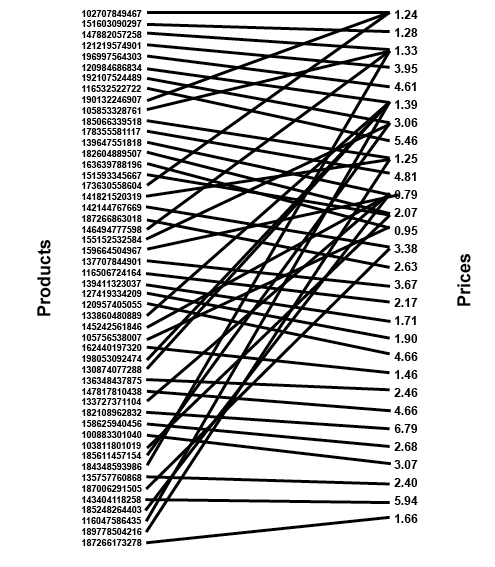
\includegraphics{pics/Product_Price_Map.png}
\end{image}




\begin{dialogue}
\item[QUESTION:] How many pairs are there in the Product-Price relation that look like (number, 2.07) ? \\
\item[ANSWER:] 2. number could be 182604889507 or 103811801019. \\
\end{dialogue}

\begin{dialogue}
\item[QUESTION:] Is it possible that a particular number is in more than one pair in the Product-Price relation? \\
\item[ANSWER:] No. Products only have one price.  Shoppers get very anxious at the cash register when this expectation breaks down. \\
\end{dialogue}

\begin{dialogue}
\item[QUESTION:] Is it possible that a particular price occurs in more than one pair in the Product-Price relation? \\
\item[ANSWER:] Yes. Two different products can have the same price.  We expect that to happen. \\
\end{dialogue}


Take a look at the map of the Product-Price relation again.  While the right side is a bit of a mess, the left side if very clean and orderly: one number, one line.  This goes back to a previous question, in which we decided that each domain GTIN number is in only one pair



This is nice. 


We like this.

\textbf{Simplifying More} \\
Let's only look at relations where each domain item occurs in exactly one pair. These types of relations are easier to examine and questions about them are easier to answer.  We can certainly return to studying all relations at a later time, but for now let's focus on these cleaner types of relations.  

These cleaner types of relations are special, so they deserve a special name.


\begin{center}
FUNCTIONS
\end{center}

\begin{definition}
A \textbf{function} is a relation in which each domain item occurs in exactly one pair.
\end{definition}

\quad \\

The Product-Price relation is now also a function, because it is a special relation where each domain product is paired with exactly one codomain price.

It doesn't go the other way, though, as the Product-Price function illustrates. Each domain product is in exactly one pair, however, a codomain price might be in multiple pairs.  We only cleaned up one side.  Maybe we?ll have to clean up the other side later, but for now we?ll just clean up the domain side.

\begin{itemize}
\item The Totman relation is not a function, because there are domain people appearing in multiple pairs.
\item Q-CLE is not a function, because there are players in the domain appearing in multiple pairs.
\end{itemize}










\end{document}
